\documentclass[conference]{IEEEtran}
\usepackage{fancyhdr}
\usepackage{multirow}
\usepackage{amsmath}
\usepackage{graphicx}
\usepackage{cite}
\usepackage{amsfonts}
\usepackage{listings}
\usepackage[colorlinks=true,
            urlcolor  = blue,
            citecolor = red]{hyperref}

\lstset{language=Python}
\setlength{\headheight}{15.2pt}
\pagestyle{fancy}
\renewcommand{\headrulewidth}{0pt} % no line in header area
\fancyhead{}
\lhead{Mini-Project \#3}
\chead{Handwritten Digits Classification}
\rhead{COMP 598}
\fancyfoot{}


\author{David Rapoport, Zafarali Ahmed, Pascale Gourdeau\\Team Name: TBD}
\title{COMP-598 Mini-Project \#3\\Handwritten Digits Classification}
\date{\today}
\begin{document}
\maketitle

\section{Introduction}
The MNIST database\ref{MnistHome} of handwritten digits is often used as a baseline to compare performance of different classifiers. In this paper, we use a modified version of the MNIST database where the digits have been modified by (1) embossing, (2) rotation, (3) rescaling, and (4) random texturing. This makes the problem much more difficult and we demonstrate poor performance with linear classifiers.

In this work we explore the performance of three classifiers: (1) Logistic Regression, (2) Support Vector Machine and (3) The Feed-forward Neural Network. 

<Something about results>


\section{Related Work}




\section{Data}
The dataset was obtained from the Kaggle Competition Website. It is a modification of the MNIST \ref{MnistHome} database. A sampling of some digits can be seen in \fig{MNISTSample} and it is aparent that this proves to be a difficult task for even humans to distinguish. In particular, we expect the digits $6$ and $9$ to be almost indistinguishable.



\begin{figure}[H]
	\centering
	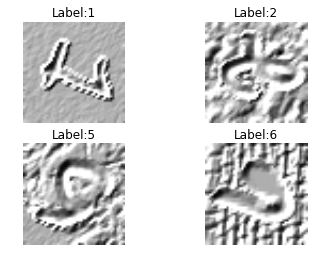
\includegraphics[scale=0.40]{sample_of_images.png}
	\caption{A sampling of the modified MNIST database}
	\label{MNISTSample}
\end{figure}

\section{Methodology}

We used the \href{http://www.numpy.org/}{NumPy package} and the \href{http://www.scikit-learn.org/}{scikit-learn library} to perform feature extraction and selection, implement our classifiers, and analyse our results. 

\subsection{Feature Extraction and Preprocessing}


\subsection{Feature Selection}

\subsection{Classification Algorithms}

\subsection{Cross-Validation and Choice of Hyperparameters}

\section{Results}




\section{Discussion}

\subsection{Feature Extraction and Selection}



\subsection{Classifier Performance}

\subsection{Future Work}



\section{Statement of Contributions}

\section{Integrity of work}
We hereby state that all the work presented in this report is that of the authors.
\begin{thebibliography}{9}

\bibitem{ML_textcat}
 Sebastini, F.
  \emph{Machine Learning in Automated Text Categorization}
  ACM Computing Surveys (CSUR) 34
  2002.

\bibitem{CNN_committees}
 Claudiu D. and Meier U. et al.
  \emph{Convolutional Neural Network Committees For Handwritten Character
Classification}
  ACM Computing Surveys (CSUR) 34
  2002.

\bibitem{STN}
 Jaderberg, M., et al.
  \emph{Spatial Transformer Networks}
  ArXiv
  2015

\bibitem{MnistHome}
LeCun Y., Cortes, C. and Burges C.J.C.
	\elph{The MNIST Database of handwritten digits}
	http://yann.lecun.com/exdb/mnist/

\end{thebibliography}

\end{document}
